\chapter{Implementacija i korisničko sučelje}
		
		
		\section{Korištene tehnologije i alati}
		
			Komunikacija u timu odvijala se uživo te preko aplikacija Whatsapp i Discord.

UML dijagrami izrađeni su u aplikaciji Astah\footnote{https://astah.net}, koja izdaje besplatnu studentsku licencu, te pomoću stranica VisualParadigm\footnote{https://online.visual-paradigm.com} i draw.io\footnote{https://app.diagrams.net}. Dijagram baze podataka izrađen je u online alatu ERDPlus \footnote{https://erdplus.com}.
Git\footnote{https://github.com} je služio kao sustav za upravljanje izvornim kodom, a udaljeni repozitorij projekta dostupan je na GitHubu.

Razvojno okruženje bio je Microsoft Visual Studio\footnote{https://visualstudio.microsoft.com}, a korišten je i uređivač koda Visual Studio Code\footnote{https://code.visualstudio.com}, Microsoftov program pogodan za izradu web aplikacija, koji, iako nije IDE, proširenjima (extensions) nudi podršku za mnoge programske jezike i alate kao što su debuggeri i intellisense.

Baza podataka izrađena je u sustavu Postgres\footnote{https://www.postgresql.org}, koji proširuje jezik SQL i ima reputaciju pouzdanog i moćnog alata za upravljanje bazama podataka, a deployana je na poslužitelju u oblaku Render\footnote{https://render.com}. 
Backend je napisan u Javi te je korišten Spring Boot\footnote{https://spring.io/projects/spring-boot}. Spring Boot je framework temeljen na Java frameworku, dizajniran da autokonfiguracijom i metodom convention-over-configuration pojednostavi izradu aplikacija. 

Za frontend je upotrebljen su standardni jezici HTML, CSS i JavaScript te React\footnote{https://react.dev}, široko upotrebljivana biblioteka za izradu web i native korisničkih sučelja, temeljena na izradni pojedinačnih, jednostavnijih komponenti koje zajedno čine složeni UI, a koju održava Meta. 

Pri izradi, to jest lokalnom testiranju, korišten je Vite\footnote{https://vitejs.dev}. Vite je lokalni server koji prati promjene u datoteci i nakon spremanja automatski osvježava browser kako bi te promjene odmah bile vidljive.

Za ostvarenje interaktivne karte i geokodiranje, korištene su usluge platforme Mapbox\footnote{https://www.mapbox.com}.
			
			\eject 
		
	
		\section{Ispitivanje programskog rješenja}
			
			
			
			 
			
			\subsection{Ispitivanje komponenti}
			     Sastavne programske komponente formirane su od nekoliko jedinica, uključujući osnovne dijelove programa poput razreda, pripadajućih metoda i atributa, koje međusobno intenzivno surađuju. Interakcija se ostvaruje kroz proceduralna sučelja, gdje svaka komponenta enkapsulira određeni skup funkcionalnosti koje druge komponente mogu pozivati. Evaluacija komponenata izvodi se s pomoću Junit radnog okvira, koji automatizira proces testiranja. Upotrebom dviju vrsta testova, jednih u uobičajenim uvjetima rada i drugih s unosom neispravnih i rubnih uvjeta, analizira se očekivano ponašanje razreda i unaprijed definirani izlaz metoda.
            Za testiranje BookService metoda koristili smo sučelja Knjiga, Pondua, i BookRepository. Prvo smo testirali saveBook metodu.
           \begin{lstlisting}[language=Java, label=lst:java_example, basicstyle=\scriptsize]
 @Test
    @DisplayName("Testiranje saveBook metode")
    void testSaveBook() {
        // Priprema podataka
        Knjiga knjiga = new Knjiga();
        List<Ponuda> ponude = new ArrayList<>();
        knjiga.setNaziv("Naslov knjige");
        knjiga.setIsbn("100");
        knjiga.setAutor("autor");
        knjiga.setIzdavac("izdavac");
        knjiga.setBrojIzdanja(1);
        knjiga.setOpis("opis");
        knjiga.setGodIzdanja(2005);
        knjiga.setSlikaURL("url");
        knjiga.setId(1L);
        knjiga.setOznaka("oznaka");
        knjiga.setKategorija("kategorija");
        knjiga.setStanjeOcuvanosti("st_oc");
        knjiga.setZahtjevi(50);
        knjiga.setZanr("zanr");
        knjiga.setPonude(ponude);


        when(bookRepository.save(any(Knjiga.class))).thenReturn(knjiga);


        Knjiga savedKnjiga = bookService.saveBook(knjiga);


        verify(bookRepository, times(1)).save(knjiga);
        assertNotNull(savedKnjiga);
        assertEquals("Naslov knjige", savedKnjiga.getNaziv());
        assertEquals("100", savedKnjiga.getIsbn());
        assertEquals("autor", savedKnjiga.getAutor());
        assertEquals("izdavac", savedKnjiga.getIzdavac());
        assertEquals(1, savedKnjiga.getBrojIzdanja());
        assertEquals("opis", savedKnjiga.getOpis());
        assertEquals(2005, savedKnjiga.getGodIzdanja());
        assertEquals("url", savedKnjiga.getSlikaURL());
        assertEquals(1L, savedKnjiga.getId());
        assertEquals("oznaka", savedKnjiga.getOznaka());
        assertEquals("kategorija", savedKnjiga.getKategorija());
        assertEquals("st_oc", savedKnjiga.getStanjeOcuvanosti());
        assertEquals(50, savedKnjiga.getZahtjevi());
        assertEquals("zanr", savedKnjiga.getZanr());
        assertNotNull(savedKnjiga.getPonude());

    }
			\end{lstlisting}

   
			A zatim smo testirali deleteBook metodu. 
                  \begin{lstlisting}[language=Java, label=2st:java_example, basicstyle=\scriptsize]
 @Test
    @DisplayName("Testiranje deleteBook metode.")
    void testDeleteBook(){
        Long bookIdToDelete = 1L;
        bookService.deleteBook(bookIdToDelete);
        verify(bookRepository).deleteById(bookIdToDelete);
    }
    
				\end{lstlisting}

            Zatim smo testirali KorisnikService. Za to smo koristili sučelja Korisnik, Ponuda, i KorisnikRepository.
            
			Prvo smo testirali dohvaćanje korisnika. 
                  \begin{lstlisting}[language=Java, label=3st:java_example, basicstyle=\scriptsize]
 @Test
    @DisplayName("Test dohvacanja korisnika.")
    void testGetUserById() {
        Long userId = 1L;
        Korisnik mockKorisnik = new Korisnik();
        List<Ponuda> ponude = new ArrayList<>();

        mockKorisnik.setId(userId);
        mockKorisnik.setUsername("username");
        mockKorisnik.setPassword("password");
        mockKorisnik.setEmail("email@gmail.com");
        mockKorisnik.setOdobren(false);
        mockKorisnik.setTip("tip");
        mockKorisnik.setAdresa("adresa");
        mockKorisnik.setTelefon("123456789");
        mockKorisnik.setPonude(ponude);
        mockKorisnik.setPrijavljen(false);
        mockKorisnik.setURLL("url");
        mockKorisnik.setNaziv("naziv");

        when(korisnikRepository.findById(userId)).thenReturn(Optional.of(mockKorisnik));

        Korisnik result = korisnikService.getUserById(userId);

        assertEquals(userId, result.getId());
        assertEquals("adresa", result.getAdresa());
        assertEquals("123456789", result.getTelefon());
        assertEquals("tip", result.getTip());
        assertEquals("email@gmail.com", result.getEmail());
        assertEquals("password", result.getPassword());
        assertEquals("username", result.getUsername());
        assertEquals(false, result.getOdobren());
        assertNotNull(ponude);
        assertEquals(false, result.isPrijavljen());
        assertEquals("url", result.getURLL());
        assertEquals("naziv", result.getNaziv());
    }

    
				\end{lstlisting}
            
			Zatim smo testirali funkcionalnost spremanja korisnika. 
                  \begin{lstlisting}[language=Java, label=4st:java_example, basicstyle=\scriptsize]
 @Test
    @DisplayName("Test spremanja korisnika.")
    void saveUserTest(){
        Long userId = 1L;
        Korisnik mockKorisnik = new Korisnik();
        List<Ponuda> ponude = new ArrayList<>();

        mockKorisnik.setId(userId);
        mockKorisnik.setUsername("username");
        mockKorisnik.setPassword("password");
        mockKorisnik.setEmail("email@gmail.com");
        mockKorisnik.setOdobren(false);
        mockKorisnik.setTip("tip");
        mockKorisnik.setAdresa("adresa");
        mockKorisnik.setTelefon("123456789");
        mockKorisnik.setPonude(ponude);
        mockKorisnik.setPrijavljen(false);
        mockKorisnik.setURLL("url");
        mockKorisnik.setNaziv("naziv");


        when(korisnikRepository.save(any(Korisnik.class))).thenReturn(mockKorisnik);

        Korisnik savedKorisnik = korisnikService.saveKorisnik(mockKorisnik);

        verify(korisnikRepository, times(1)).save(mockKorisnik);
        
        assertEquals(userId, savedKorisnik.getId());
        assertEquals("adresa", savedKorisnik.getAdresa());
        assertEquals("123456789", savedKorisnik.getTelefon());
        assertEquals("tip", savedKorisnik.getTip());
        assertEquals("email@gmail.com", savedKorisnik.getEmail());
        assertEquals("password", savedKorisnik.getPassword());
        assertEquals("username", savedKorisnik.getUsername());
        assertEquals(false, savedKorisnik.getOdobren());
        assertNotNull(ponude);
        assertEquals(false, savedKorisnik.isPrijavljen());
        assertEquals("url", savedKorisnik.getURLL());
        assertEquals("naziv", savedKorisnik.getNaziv());
    }
    
\end{lstlisting}
            
			Nakon toga smo testirali ponudu, to jest OfferService. Za te testove smo koristili sučelja Knjiga, Korisnik, Ponuda, PonudaDto, BookRepository, KorisnikRepository, OfferRepository i OfferService. 
            Prvo smo testirali brisanje ponude. 
            
                  \begin{lstlisting}[language=Java, label=5st:java_example, basicstyle=\scriptsize]
 @Test
    @DisplayName("Testiranje brisanja ponude.")
    void deleteOfferTest() {
        Long offerId = 1L;

        offerService.deleteOffer(offerId);

        verify(offerRepository, times(1)).deleteById(offerId);
    }
    
\end{lstlisting}
            A zatim smo testirali spremanje ponude. 
                  \begin{lstlisting}[language=Java, label=6st:java_example, basicstyle=\scriptsize]
  @Test
    @DisplayName("Testiranje spremanja ponude.")
    void saveOffer() {
        // Arrange
        PonudaDto ponudaDto = new PonudaDto();
        ponudaDto.setPonuditeljId(1L);
        ponudaDto.setKnjigaId(2L);
        ponudaDto.setCijena(100);
        ponudaDto.setBrojPrimjeraka(5);

        Korisnik mockKorisnik = new Korisnik();
        Knjiga mockKnjiga = new Knjiga();
        Ponuda mockPonuda = new Ponuda();

        when(korisnikRepository.findById(ponudaDto.getPonuditeljId())).thenReturn(java.util.Optional.of(mockKorisnik));
        when(bookRepository.findById(ponudaDto.getKnjigaId())).thenReturn(java.util.Optional.of(mockKnjiga));
        when(offerRepository.save(any(Ponuda.class))).thenReturn(mockPonuda);


        Ponuda resultPonuda = offerService.saveOffer(ponudaDto);

        verify(offerRepository).save(any(Ponuda.class));

        assertEquals(mockPonuda, resultPonuda);
    }

    
\end{lstlisting}
            Zatim smo testirali kada spremamo ponudu, a ne postoji taj userId.
                  \begin{lstlisting}[language=Java, label=7st:java_example, basicstyle=\scriptsize]
 @Test
    @DisplayName("Testiranje kada spremamo ponudu. a ne postoji taj userId.")
    void saveOfferInvalid() {
        PonudaDto ponudaDto = new PonudaDto();
        ponudaDto.setPonuditeljId(1L);
        ponudaDto.setKnjigaId(2L);
        ponudaDto.setCijena(100);
        ponudaDto.setBrojPrimjeraka(5);

        when(korisnikRepository.findById(ponudaDto.getPonuditeljId())).thenReturn(Optional.empty());

        // Act & Assert
        // Verify that ResponseStatusException is thrown with the correct status and message
        ResponseStatusException exception = Assertions.assertThrows(ResponseStatusException.class, () -> {
            offerService.saveOffer(ponudaDto);
        });

        assertEquals(HttpStatus.NOT_FOUND, exception.getStatusCode());
        assertEquals("Korisnik not found", exception.getReason());
    }
    
\end{lstlisting}

            Svi testovi su se ispravno izveli s očekivanim rezultatima. 
          
			
			
			\begin{figure}[H]
				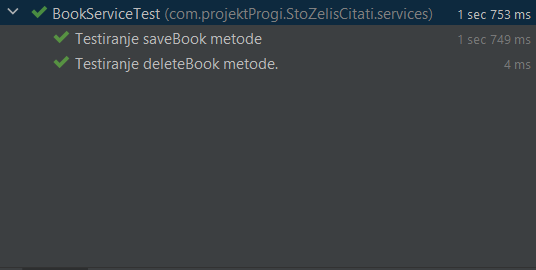
\includegraphics[width=\textwidth]{slike/UnitTest1.PNG} %veličina u odnosu na širinu linije
				\centering
				\caption{Rezultat testiranja BookService }
				\label{fig:BookService1}
			\end{figure}
			
			
			
			\begin{figure}[H]
				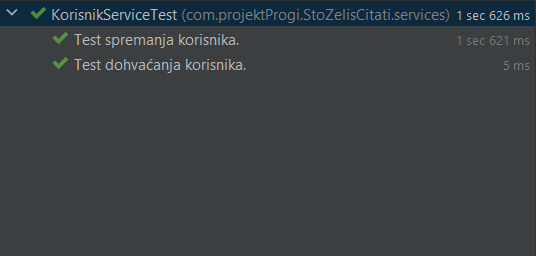
\includegraphics[width=\textwidth]{slike/UnitTest3.PNG} %veličina u odnosu na širinu linije
				\centering
				\caption{Rezultat testiranja KorisnikService }
				\label{fig:KorisnikService1}
			\end{figure}
			
			
			
			\begin{figure}[H]
				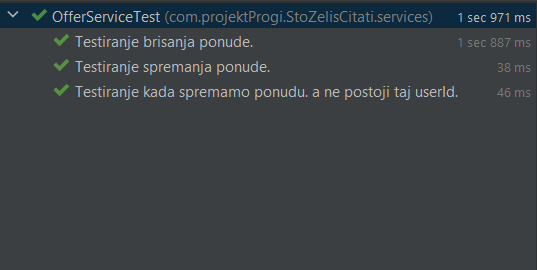
\includegraphics[width=\textwidth]{slike/UnitTest2.PNG} %veličina u odnosu na širinu linije
				\centering
				\caption{Rezultat testiranja OfferService}
				\label{fig:OfferService1}
			\end{figure}
			
			\eject
			
			
			
			
			
			\subsection{Ispitivanje sustava}
			
			 Testiranje cjelokupnog sustava obavljeno je korištenjem Selenium WebDriver-a unutar JUnit testova. U svakom od testova unaprijed postavljamo konfiguraciju drivera, uključujući URL aplikacije. Zatim driver automatski locira prethodno definirane elemente, a test mu proslijeđuje potrebne podatke.
    
            Prvo smo testirali logiranje već prije registriranog korisnika.
           \begin{lstlisting}[language=Java, label=8st:java_example, basicstyle=\scriptsize9]
 public class SeleniumTest1 {
    public static void main(String[] args) {
        System.setProperty("webdriver.chrome.driver", "C:\\Faks\\TrecaGod\\PROGI\\Projekt\\chromedriver-win64\\chromedriver.exe");
        WebDriver webDriver = new ChromeDriver();
        webDriver.manage().timeouts().implicitlyWait(10L, TimeUnit.SECONDS);
        boolean result = loginTest(webDriver, "user", "pass");
        System.out.println("Test pass: " + result);

        WebDriver webDriver2 = new ChromeDriver();
        webDriver2.manage().timeouts().implicitlyWait(10L, TimeUnit.SECONDS);
        result = loginTest(webDriver2, "kriviuser", "krivasifra");
        System.out.println("Test pass: " + result);
        webDriver.quit();
        webDriver2.quit();
    }

    public static boolean loginTest(WebDriver driver, String username, String password){

        try {
            driver.get("http://localhost:5173/login/");
            WebElement element = driver.findElement(By.name("username"));
            element.sendKeys(new CharSequence[]{username});
            element = driver.findElement(By.name("password"));
            element.sendKeys(new CharSequence[]{password});
            driver.findElement(By.name("submit")).click();
        }catch (UnhandledAlertException e){
        }

        try {
            Thread.sleep(5000);
        } catch (InterruptedException e) {
            e.printStackTrace();
        }
        String redirectionURL = driver.getCurrentUrl();
        System.out.println("Trenutni URL je: " + redirectionURL);

        return redirectionURL.contains("user");
    }
\end{lstlisting}

   
			Zatim smo testirali registraciju novoga korisnka.
                  \begin{lstlisting}[language=Java, label=9st:java_example, basicstyle=\scriptsize]
 public class SeleniumTest2 {
    public static void main(String[] args) {
        System.setProperty("webdriver.chrome.driver", "C:\\Faks\\TrecaGod\\PROGI\\Projekt\\chromedriver-win64\\chromedriver.exe");
        WebDriver webDriver = new ChromeDriver();
        webDriver.manage().timeouts().implicitlyWait(10L, TimeUnit.SECONDS);
        boolean result = registerTest(webDriver, "user", "pass", "naziv", "adresa", "tel", "mail@gmail.com",
                "antikvarijat");
        System.out.println("Test pass " + result);
        webDriver.quit();
    }

    public static boolean registerTest(WebDriver driver, String username, String password, String naziv, String adresa, String telefon,
        String email, String tip){
        String redirectionURL = "";
        try{ driver.get("http://localhost:5173/register/");
            WebElement element = driver.findElement(By.name("username"));
            element.sendKeys(new CharSequence[]{username});
            element = driver.findElement(By.name("password"));
            element.sendKeys(new CharSequence[]{password});
            element = driver.findElement(By.name("naziv"));
            element.sendKeys(new CharSequence[]{naziv});
            element = driver.findElement(By.name("adresa"));
            element.sendKeys(new CharSequence[]{adresa});
            element = driver.findElement(By.name("telefon"));
            element.sendKeys(new CharSequence[]{telefon});
            element = driver.findElement(By.name("email"));
            element.sendKeys(new CharSequence[]{email});
            driver.findElement(By.name("tip")).click();
            driver.findElement(By.name(tip)).click();
            driver.findElement(By.name("submit")).click();
        } catch (UnhandledAlertException e){
                System.out.println(e.getAlertText());
        }

        try {
            Thread.sleep(5000);
        } catch (InterruptedException e) {
            e.printStackTrace();
        }
        redirectionURL = driver.getCurrentUrl();
        System.out.println("Trenutni URL je: " + redirectionURL);
        return redirectionURL.contains("login");
    }
    
\end{lstlisting}

			Nakon toga testiramo ulogiravanje registriranog korisnika, te nakon ulogiravanja dodajemo knjigu.
                  \begin{lstlisting}[language=Java, label=l0st:java_example, basicstyle=\scriptsize]
 public class SeleniumTest3 {
    public static void main(String[] args) {
        System.setProperty("webdriver.chrome.driver", "C:\\Faks\\TrecaGod\\PROGI\\Projekt\\chromedriver-win64\\chromedriver.exe");
        WebDriver webDriver = new ChromeDriver();
        String oznaka = "hrv+dobavljiva";
        String kategorija = "domaci";
        String stanje = "izvrsno";
        webDriver.manage().timeouts().implicitlyWait(10L, TimeUnit.SECONDS);
        boolean result = addBookTest(webDriver, "user", "pass", "naziv", "autor", "izdavac", kategorija,
                "zanr", "opis", oznaka, "url", "2005", "1", stanje);
        System.out.println("Test pass " + result);
        webDriver.quit();
    }

    private static boolean addBookTest(WebDriver driver, String username, String password, String naziv, String autor, String izdavac, String kategorija,
                                       String zanr, String opis, String oznaka, String url, String godina, String broj, String stanje){
        driver.get("http://localhost:5173/login/");
        WebElement element = driver.findElement(By.name("username"));
        element.sendKeys(new CharSequence[]{username});
        element = driver.findElement(By.name("password"));
        element.sendKeys(new CharSequence[]{password});
        driver.findElement(By.name("submit")).click();
        try {
            Thread.sleep(5000);
        } catch (InterruptedException e) {
            e.printStackTrace();
        }
        String redirectionURL = driver.getCurrentUrl();
        System.out.println("Trenutni URL je: " + redirectionURL);

        driver.findElement(By.name("addButton")).click();

        element = driver.findElement(By.name("naziv"));
        element.sendKeys(new CharSequence[]{naziv});
        element = driver.findElement(By.name("autor"));
        element.sendKeys(new CharSequence[]{autor});
        element = driver.findElement(By.name("izdavac"));
        element.sendKeys(new CharSequence[]{izdavac});
        element = driver.findElement(By.name("zanr"));
        element.sendKeys(new CharSequence[]{zanr});
        element = driver.findElement(By.name("opis"));
        element.sendKeys(new CharSequence[]{opis});
        element = driver.findElement(By.name("slikaURL"));
        element.sendKeys(new CharSequence[]{url});
        element = driver.findElement(By.name("godIzdanja"));
        element.sendKeys(new CharSequence[]{godina});
        element = driver.findElement(By.name("brojIzdanja"));
        element.sendKeys(new CharSequence[]{broj});

        driver.findElement(By.name("kategorija")).click();
        driver.findElement(By.name(kategorija)).click();

        driver.findElement(By.name("oznaka")).click();
        driver.findElement(By.name(oznaka)).click();

        driver.findElement(By.name("stanjeOcuvanosti")).click();
        driver.findElement(By.name(stanje)).click();

        driver.findElement(By.name("submit")).click();
        try {
            Thread.sleep(5000);
        } catch (InterruptedException e) {
            e.printStackTrace();
        }
        String redirectURL = driver.getCurrentUrl();
        System.out.println("Trenutni URL je: " + redirectURL);
        return redirectURL.contains("user");

    }    
\end{lstlisting}
            
			Te za kraj smo testirali unošenje zahtjeva za prevođenje knjige.
                  \begin{lstlisting}[language=Java, label=l1st:java_example, basicstyle=\scriptsize]
 public class SeleniumTest4 {
    public static void main(String[] args) {
        System.setProperty("webdriver.chrome.driver", "C:\\Faks\\TrecaGod\\PROGI\\Projekt\\chromedriver-win64\\chromedriver.exe");
        WebDriver webDriver = new ChromeDriver();
        webDriver.manage().timeouts().implicitlyWait(10L, TimeUnit.SECONDS);
        boolean result = testTranslationRequest(webDriver,"naziv");
        System.out.println("Test pass " + result);
        webDriver.quit();
    }

    private static boolean testTranslationRequest(WebDriver driver, String naziv){
        driver.get("http://localhost:5173/");
        driver.findElement(By.className("request_translation")).click();
        WebElement element = driver.findElement(By.name("naziv"));
        element.sendKeys(new CharSequence[]{naziv});
        driver.findElement(By.name("submit")).click();
        try {
            Thread.sleep(10000);
        } catch (InterruptedException e) {
            e.printStackTrace();
        }
        String redirectURL = driver.getCurrentUrl();
        System.out.println("Trenutni URL je: " + redirectURL);

        return redirectURL.equals("http://localhost:5173/");
    }
    
\end{lstlisting}
            
			

            Svi testovi su se ispravno izveli s očekivanim rezultatima. 
            
			
			
			\begin{figure}[H]
				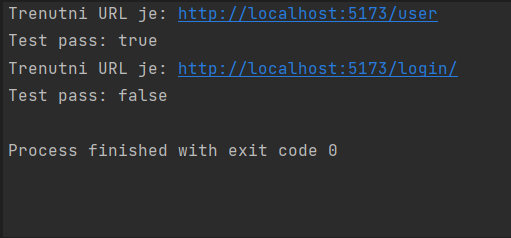
\includegraphics[width=\textwidth]{slike/SelTest1.PNG} %veličina u odnosu na širinu linije
				\centering
				\caption{Rezultat testiranja logina }
				\label{fig:loginTest1}
			\end{figure}
			
			
			
			\begin{figure}[H]
				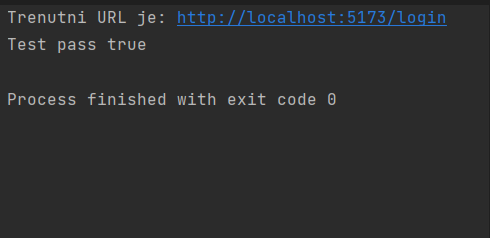
\includegraphics[width=\textwidth]{slike/SelTest2.PNG} %veličina u odnosu na širinu linije
				\centering
				\caption{Rezultat testiranja registriranja }
				\label{fig:registerTest1}
			\end{figure}
			
			
			
			\begin{figure}[H]
				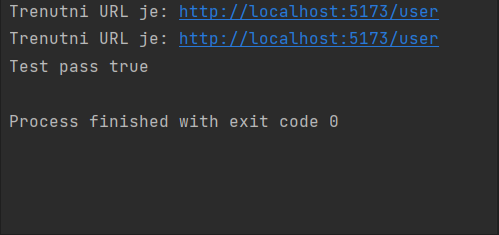
\includegraphics[width=\textwidth]{slike/SelTest3.PNG} %veličina u odnosu na širinu linije
				\centering
				\caption{Rezultat testiranja logina uz dodavanje knjige}
				\label{fig:addBookTest1}
			\end{figure}
			
			
			
			\begin{figure}[H]
				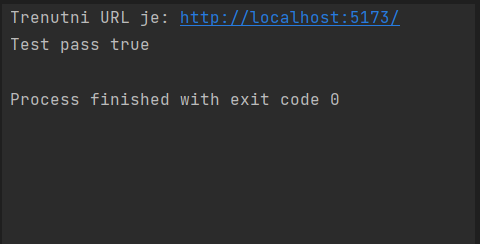
\includegraphics[width=\textwidth]{slike/SelTest4.PNG} %veličina u odnosu na širinu linije
				\centering
				\caption{Rezultat testiranja dodavanje zahtjeva za prevođenje}
				\label{fig:testTranslationRequest1}
			\end{figure}
			
			\eject
		
		
		
		\section{Dijagram razmještaja}
			
			Dijagrami razmještaja prikazuju fizičku arhitekturu i topologiju programskog sustava te programsku potporu koja se koristi u njegovom radnom okruženju. Na korisničkom računalu se nalazi web preglednik koji služi za pristupanje web aplikaciji. Na poslužiteljskom računalu se nalaze web poslužitelj i poslužitelj baze podataka koji međusobno komuniciraju. Sustav koristi arhitekturu "klijent - poslužitelj", a komunikacija između korisnika(klijent, izdavač, administrator) i poslužitelja se odvija preko HTTP protokola.
			
			\begin{figure}[H]
				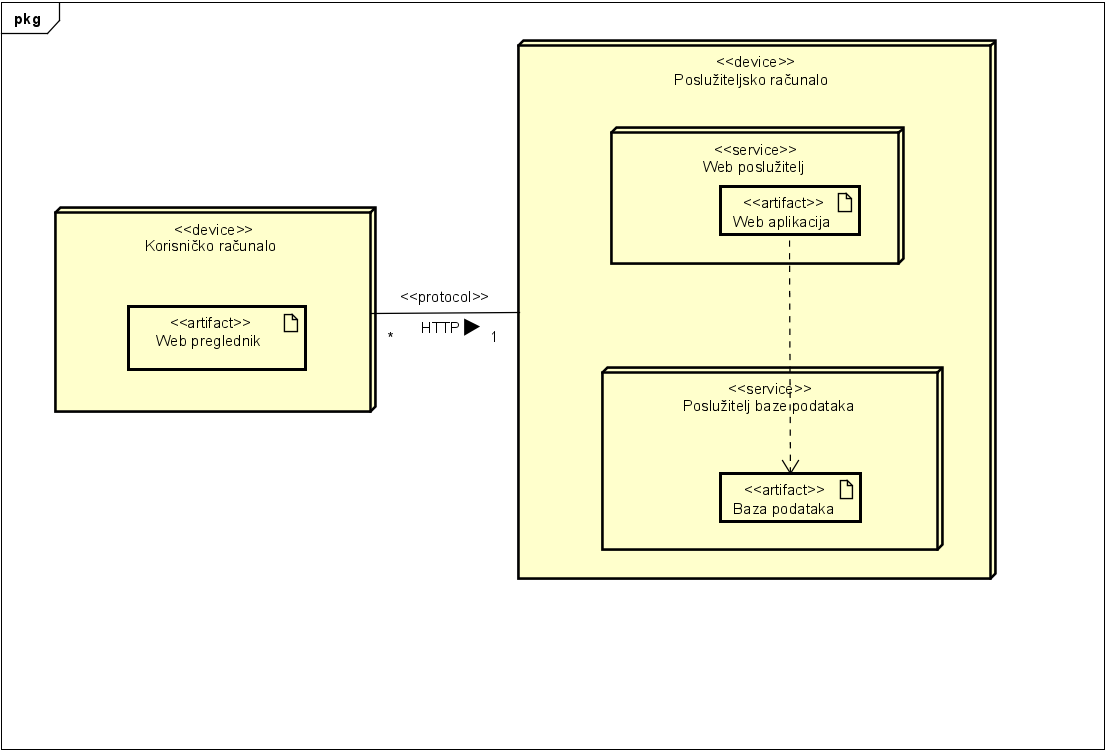
\includegraphics[width=\textwidth]{dijagrami/DijagramRazmjestaja.PNG} %veličina u odnosu na širinu linije
				\centering
				\caption{Dijagram razmještaja}
				\label{fig:diagrazmjestaja}
			\end{figure}
			
			
			\eject 
		
		\section{Upute za puštanje u pogon}
		
			
            Za deploy cjelokupne aplikacije 	korištena je usluga Render čime je omogućeno da aplikacija bude javno dostupna. Backend aplikacije je napisan u Springboot-u te smo koristili IDE IntelliJ.  Frontend je napisan s pomoću tehnologije React.js te je pisan u JavaScriptu. Baza podataka se nalazi na javnom Render serveru. \\

            \textbf{Konfiguracija Backenda:}
            
            S pomoću IDE Intellij je ostvarena backend podrška, te se radi o Maven projektu.
            Da bi se lokalno pokrenulo na računalu potrebno je instalirati Maven dependecies (Intellij ovo radi automatski pri pokretanju projekta).
            Stoga je potrebno kliknuti \textit{run/build project} te će se backend automatski povezati s bazom podataka.
            Nakon toga je potrebno pokrenuti frontend. \\

            \textbf{Konfiguracija Frontenda:}
            
            Što se tiče frontenda potrebno je imati instaliran Node.js (preporučljiva najnovija verzija). 
            Da bi se stranica pokrenula na localhostu prvo je potrebno pozicionirati se u direktorij "frontend" te utipkati u terminal  
                \textit{npm install.}
         
			
			
			\begin{figure}[H]
				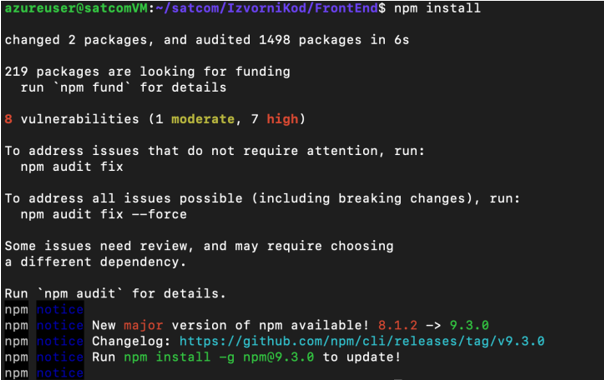
\includegraphics[width=\textwidth]{slike/npm install.PNG} %veličina u odnosu na širinu linije
				\centering
				\caption{Prikaz terminala nakon unosa naredbe \textit{npm install} }
				\label{fig:npminstall1}
			\end{figure}
			
			
 	
            Te nakon toga u terminal napisati: 
            \textit{npm run dev.}
            Ovo će pokrenuti React.js frontend dio aplikacije koristeći najnoviju verziju VITE-a na default \textit{localhostu:5137}
